\documentclass[a4j,20pt,slide]{ltjsarticle}
% \usepackage[ipa]{luatexja-preset}
\usepackage{amsmath}
\usepackage[table]{xcolor}
\usepackage{graphicx}
\graphicspath{{./fig/}}
\usepackage{url}
\usepackage{listings}
\usepackage[pdfencoding=auto]{hyperref}
\hypersetup{
  bookmarksnumbered=true,
  colorlinks=true,
  pdftitle={Salome-Mecaで超弾性材料を使ってみた!},
  pdfsubject={第19回オープンCAE勉強会@関東(構造など)},
  pdfauthor={龍野 潤 (@Jun_Tatsuno)(オープンCAE学会・CAE懇話会)}
}
\usepackage{here}
\usepackage{booktabs}
\usepackage{menukeys}
\renewmenumacro{\directory}{pathswithfolder}
\usepackage[labelformat=empty,labelsep=none]{caption}
% \usepackage{geometry}
% \geometry{textwidth=270mm, textheight=195mm}
%箇条書きの記号変更
\renewcommand{\labelitemii}{$\circ$}
\renewcommand{\labelitemiii}{$\triangleright$}
\renewcommand{\labelitemiv}{$\Rightarrow$}
%ソースコードオプション
\usepackage{listings}%ソースコード
\lstset{
language=Python, %言語
backgroundcolor={\color[gray]{.97}},%背景色
basicstyle={\footnotesize\ttfamily},
commentstyle=\color{blue},
rulecolor=\color{black},
keywordstyle={\small\bfseries \color{red}},
ndkeywordstyle={\small},
stringstyle={\small\ttfamily \color{red}},
numberstyle={\scriptsize},
frame=single, %枠線
numbers=left, %行番号を振る
breaklines=true, %長い行を折り返す
tabsize=2 %タブ幅
}
\title{「Salome-Mecaで超弾性材料を使ってみた!」\\第19回オープンCAE勉強会@関東(構造など)}
\author{龍野 潤 (@Jun\_Tatsuno)}
\date{2020年9月12日}
\pagestyle{plain}
%
\begin{document}
\maketitle
\thispagestyle{plain}
\tableofcontents
%
\section{自己紹介}
\begin{itemize}
	\item 職業:オフィス家具メーカーに勤務の会社員で2003年~CAEを担当
	\item オープンCAE歴
	      \begin{itemize}
		      \item 2011年05月:第32回関西CAE懇話会「CAEの新しい波、オープンソースとFOCUSスパコン」でオープンCAEを知る
		            \begin{itemize}
			            \item 実習講座「オープンCAEから始める構造解析CAEの基本」に参加し、岐阜高専の柴田先生、DEXCS、Adventureを知る
		            \end{itemize}
		      \item 2011年08月:関西地区の解析塾「はじめてのオープンCAE」を受講し、Salome-Mecaを知る
		      \item 2011年11月:CAE懇話会の「Salome-Meca活用研究会」が発足、参加
		      \item 2012年08月:第16回「オープンCAE勉強会@岐阜(夏合宿2)」に初参加
		      \item 2012年XX月:「オープンCAE学会」に入会
		      \item 2013年02月:第20回「オープンCAE勉強会@関西」に初参加
		      \item 2016年10月:第09回「オープンCAE勉強会@関東(構造など)」に初参加
	      \end{itemize}
	\item 情報発信
	      \begin{itemize}
		      \item Twitter \href{https://twitter.com/Jun_Tatsuno}{@Jun\_Tatsuno}
		      \item Qiita \href{https://qiita.com/Jun_Tatsuno}{@Jun\_Tatsuno}
		      \item GitHub \href{https://github.com/JunTatsuno/}{@JunTatsuno}
		      \item Speaker Deck \href{https://speakerdeck.com/juntatsuno/}{@JunTatsuno}
		      \item \href{https://www.youtube.com/playlist?list=PL3Ey4GcIvUy-2_ZMZ7dG_Wez4H__rin5c}{YouTube}
	      \end{itemize}
\end{itemize}
\section{超弾性(Hyperelasticity)}
\subsection{超弾性とは}
\begin{itemize}
	\item 物体を構成する物質の力学的特性の数理的表現のひとつ
	\item ひずみエネルギー密度関数(単位体積あたりのひずみエネルギーを表す弾性ポテンシャル)を有することが特徴
	\item 超弾性を有する物質を超弾性体とよび、ゴムの最も簡易なモデルとして登場したことに由来して、数10 %~数100%の大ひずみ状態を想定
\end{itemize}
\vspace{-\baselineskip}
\begin{flushright}
	\href{https://ja.wikipedia.org/wiki/%E8%B6%85%E5%BC%BE%E6%80%A7}{Wikipedia「超弾性」より}
\end{flushright}
\vspace{-\baselineskip}
\subsection{ゴム材料(エラストマ)の単軸引張試験結果}
\vspace{-\baselineskip}
\begin{figure}[H]
	\caption{単軸引張試験の例}
	\label{fig:002}
	\centering
	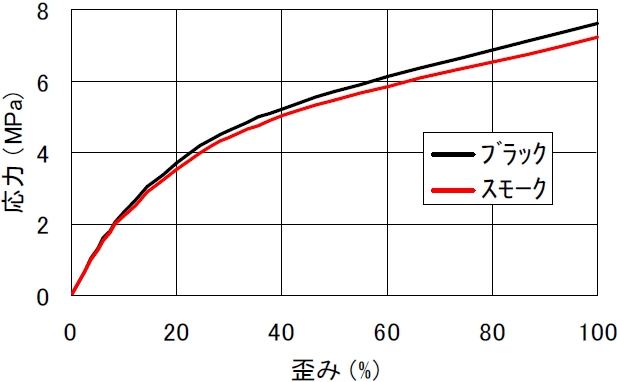
\includegraphics[width=0.4\columnwidth]{fig/tensile test.png}
\end{figure}
\section{Code\_Asterの超弾性材料}
\subsection{Code\_Asterで採用されている超弾性材料}
\begin{itemize}
	\item Signorini(シニョリーニ)
	\item Mooney-Rivlin(ムーニー・リブリン)
	\item Néo-Hookéen(ネオ・ファッキアン)
\end{itemize}
\begin{itemize}
	\item 商用ソフトにあるような以下の材料モデルには未対応
	      \begin{itemize}
		      \item Polynominal(多項式)
		      \item Yeoh(ヨー)
		      \item Ogden(オクデン)
		      \item Arruda-Boyce(アルーダ・ボイス)
		      \item Gent(ジェント)
		      \item Blatz-Ko(ブラッツ・コウ)
	      \end{itemize}
\end{itemize}
\clearpage
\subsection{キーワード因子ELAS\_HYPER}
材料を特徴づけるパラメータは、\textit{DEFI\_MATERIAU}で\textit{ELAS\_HYPER}というキーワードで定義されています。
\vspace{\baselineskip}
大きな変位、回転、および変形 (\textit{DEFORMATION=' GROT\_GDEP'}) をサポートしています。\footnote{この挙動では、熱による変形を考慮することはできません。}
\begin{itemize}
	\item 対応要素:\textit{3D}(3次元)、\textit{D\_PLAN}(平面ひずみ)、\textit{C\_PLAN}(平面応力)
	\item Example:テストケース\textit{SSNV187}
	\item Reference material \textit{R5.03.19}
\end{itemize}
\clearpage
\subsection{ELAS\_HYPER構文}
\begin{lstlisting}[caption =Syntax, label = Syntax]
| ELAS_HYPER= _F (
               ♦   C10   =   c10,     [R]
               ◇   C01   =   / c01,   [R]
                             / 0.0,    [DEFECT]
               ◇   C20   =   / c20,   [R]
                             / 0.0,    [DEFECT]
               ◇   RHO   =   / rho,   [R]
                             / 0.0,    [DEFECT]
               ◇   NAKED =   naked,   [R]
               ◇   K     =   K        [R]
               )
\end{lstlisting}
\clearpage
\subsubsection{オペランド\textit{C01}、\textit{C10}、\textit{C20}}
\textit{C01 = c01} 、\textit{ C10 = c10}、 \textit{C20 = c20}
超弾性多項式の3つのポテンシャル関数。\\
単位は$N/mm^{2}$
\begin{itemize}
	\item \textit{C20}のみがNullの場合、Mooney-Rivlin(ムーニー・リブリン)型の材料モデル。
	\item \textit{C01}と\textit{C20}がNullの場合、Néo-Hookéen(ネオ・ファッキアン)型の材料モデル。
\end{itemize}
\textit{6(C01+C10)=E}のように\textit{C10}と\textit{C01}を取る場合、小さな変形では弾性非圧縮性を持つ材料となります。
ここで、\textit{E}はヤング率です。
\vspace{\baselineskip}
\begin{table}[H]
	\centering
	\begin{tabular}{@{}cccc@{}}
		\toprule
		              & \textit{C01} & \textit{C10} & \textit{C20} \\ \midrule
		Signorini     & YES          & YES          & YES          \\
		Mooney-Rivlin & YES          & YES          & Null         \\
		Néo-Hookéen   & Null         & YES          & Null         \\ \bottomrule
	\end{tabular}
\end{table}
\clearpage
\subsubsection{オペランド\textit{NAKED}と\textit{K}}
\textit{NAKED = naked}\\
ポアソン比。
-1<$\nu$<0.5であることを確認します。
\textit{K = K}\\
体積弾性率。
これらの2つのパラメータは1つだけを用い、もう1つを除外します。\\
これらのパラメータは、材料の圧縮性をほぼ定量化します。\\
ユーザが提供する体積弾性率\textit{K}が存在すれば、それを使用します。\\
存在しない場合は、次式(\ref{compressibility})を用いて計算します。
\begin{equation}
	\label{compressibility}
	K=\frac{6(C01+C10)}{3(1-2\nu)}
\end{equation}
$\nu$は0.5に近い値を取ることができますが,厳密には決して等しくはありません。\\
$\nu$が0.5に近すぎる場合、ポアソン比またはその体積弾性率をチェックするように、エラーメッセージが表示されます。\\
体積弾性率が大きいほど、材料は非圧縮性が高くなります。
\subsubsection{オペランド\textit{RHO}}
\textit{RHO = rho}\\
質量密度(関数型の概念を受けつけません)。
サイズについてのチェックはありません。
\section{単純モデルでの解析}
単純モデルでの解析は、Code\_Aster 10で記述されたCAELinuxの投稿をCode\_Aster 14で実施しました。
\vspace{-\baselineskip}
\subsection{ジオメトリ}
5(mm)×12(mm)×43(mm)のブロック形状を使用
\begin{itemize}
	\item 上下の2つのエリア:AtopとAbot
	\item 2節点グループ
	      \begin{itemize}
		      \item 底面の中心節点:Nfixx
		      \item y軸の最端位置にある2つの節点:Nfixy
	      \end{itemize}
\end{itemize}
\vspace{-\baselineskip}
\begin{figure}[htbp]
	\caption{ブロック上に定義された4つのグループ}
	%\label{fig:}
	\centering
	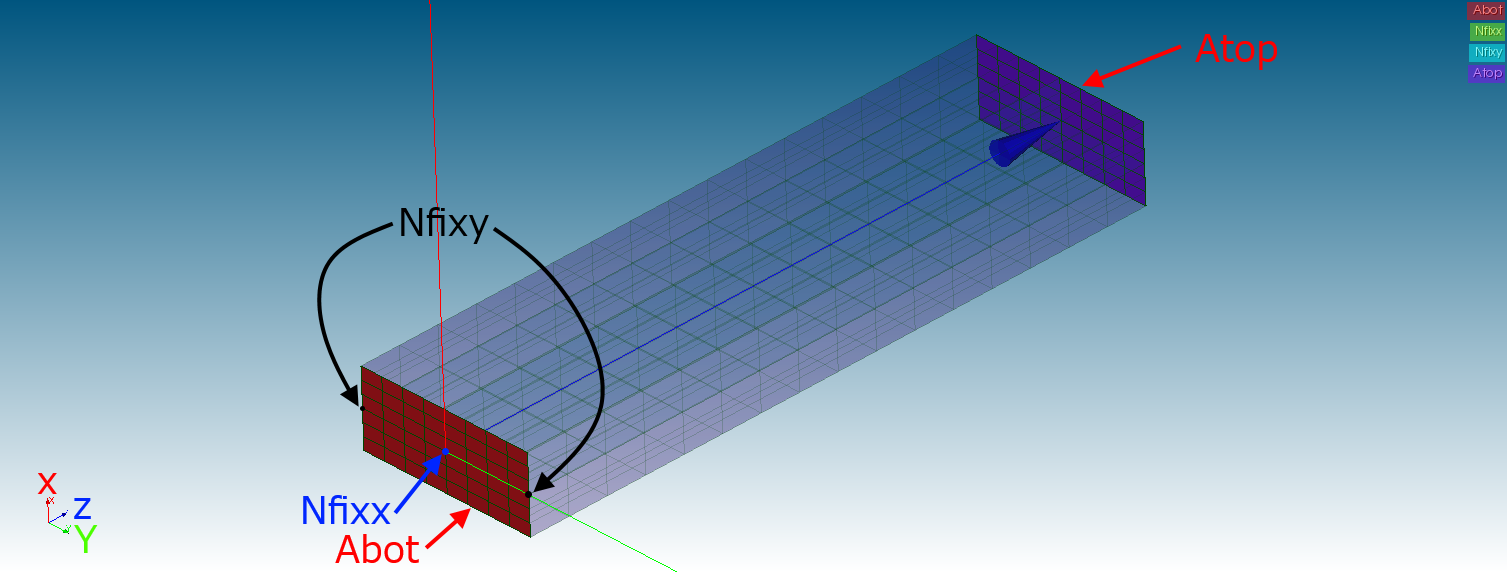
\includegraphics[width=0.7\columnwidth]{fig/bc.png}
\end{figure}
\clearpage
\subsection{コマンド}
材料特性は、Mooney-Rivlin(ムーニー・リブリン)型の材料モデルで設定しています。
\begin{lstlisting}[caption =材料設定, label=材料設定]
mater = DEFI_MATERIAU(ELAS_HYPER=_F(C01=2.3456,
                                    C10=0.709,
                                    C20=0.0,
                                    NU=0.499))
\end{lstlisting}
\begin{lstlisting}[caption =拘束条件, label=拘束条件]
mecabc = AFFE_CHAR_MECA(DDL_IMPO=(_F(DZ=0.0,
                                     GROUP_MA=('Abot', )),
                                  _F(DY=0.0,
                                     GROUP_NO=('Nfixx', )),
                                  _F(DX=0.0,
                                     GROUP_NO=('Nfixy', ))),
                        MODELE=model)
\end{lstlisting}
\begin{lstlisting}[caption =荷重条件, label=荷重条件]
mecach = AFFE_CHAR_MECA(MODELE=model,
                        PRES_REP=_F(GROUP_MA=('Atop', ),
                                    PRES=-6.0))
\end{lstlisting}
\clearpage
\begin{lstlisting}[caption =非線形解析コマンド, label=非線形解析コマンド]
resnonl = STAT_NON_LINE(CHAM_MATER=fieldmat,
                        COMPORTEMENT=_F(DEFORMATION='GROT_GDEP',
                                        RELATION='ELAS_HYPER'),
                        CONVERGENCE=_F(ITER_GLOB_MAXI=20),
                        EXCIT=(_F(CHARGE=mecabc),
                               _F(CHARGE=mecach,
                                  FONC_MULT=func)),
                        INCREMENT=_F(LIST_INST=listr),
                        MODELE=model,
                        NEWTON=_F(REAC_ITER=1))
\end{lstlisting}
\clearpage
\subsection{結果}
\subsubsection{変位}
上のエリアAtopに-6(MPa)の圧力荷重を20等分してかけています。\\
次の左図は、この荷重の全体的な変位を示しています。\\表示されている変位は、実際の変位です(デフォルメ表示はしていません)。\\
最終的なZ方向変位は34.4(mm)で、ひずみは34.4÷43=0.8($\epsilon$)です。\\
右図は圧力-12(MPa)のときのZ方向変位を示しています。\\
上面の最大変位は182.5(mm) で、ひずみは182.5÷43=4.2($\epsilon$)です。
\begin{figure}[H]
	\begin{minipage}{0.48\hsize}
		\caption{圧力荷重-6(MPa)の場合}
		%\label{}
		\centering
		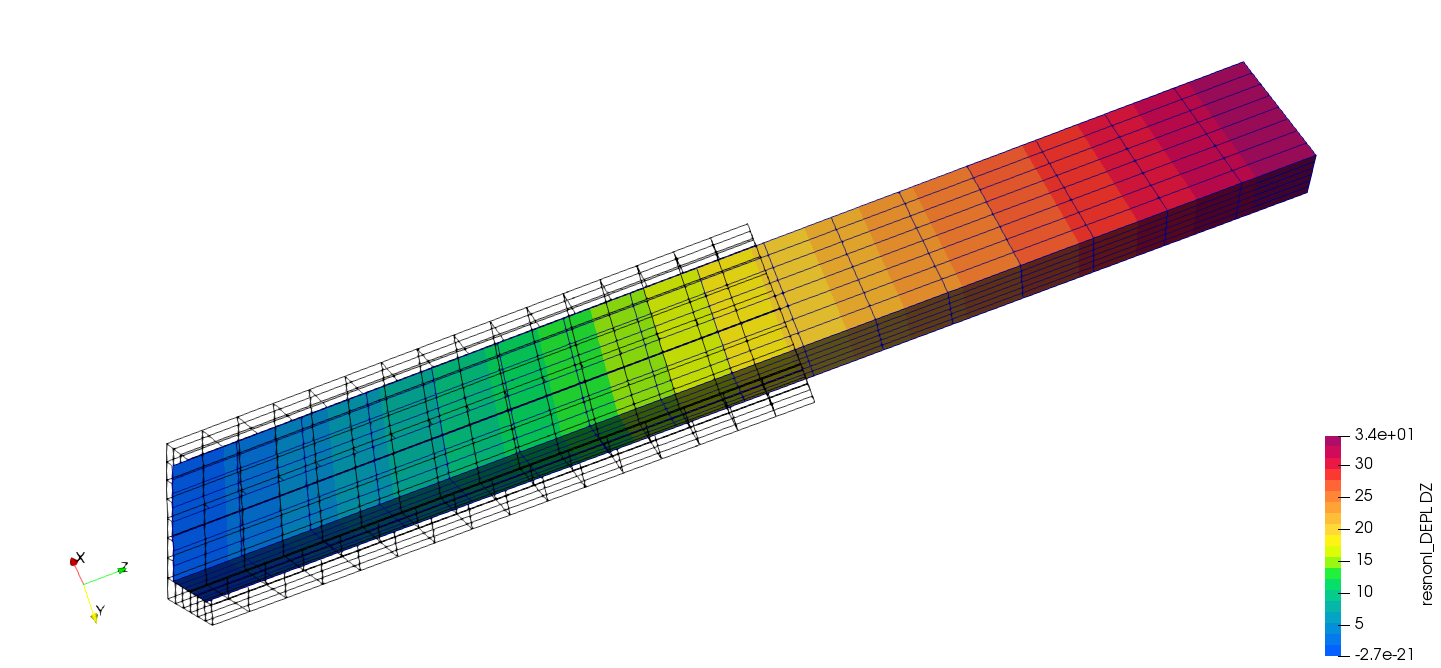
\includegraphics[width=0.9\columnwidth]{fig/6MPa.png}
	\end{minipage}
	\begin{minipage}{0.48\hsize}
		\caption{圧力荷重-12(MPa)の場合}
		%\label{}
		\centering
		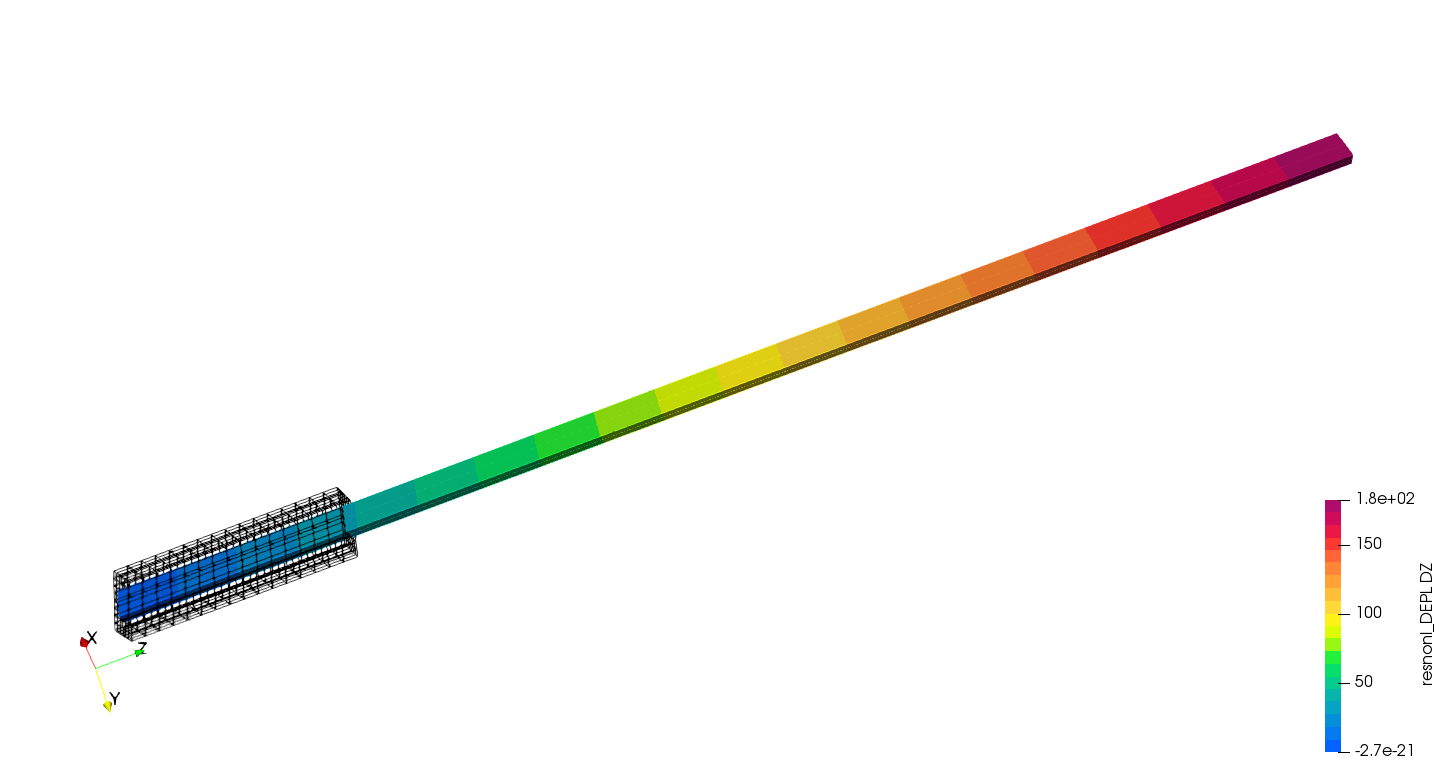
\includegraphics[width=0.9\columnwidth]{fig/12MPa.png}
	\end{minipage}
\end{figure}
\clearpage
\subsubsection{体積変化}
ここでは、-6(MPa)の圧力荷重の場合について説明します。\\
次の図は、X、Y、Z方向の変位量を示しています。\\
各方向の最大変位量は次のとおりです。
\begin{figure}[H]
	\begin{minipage}{0.32\hsize}
		\caption{X方向変位量:0.64(mm)\\(両方向)}
		%\label{}
		\centering
		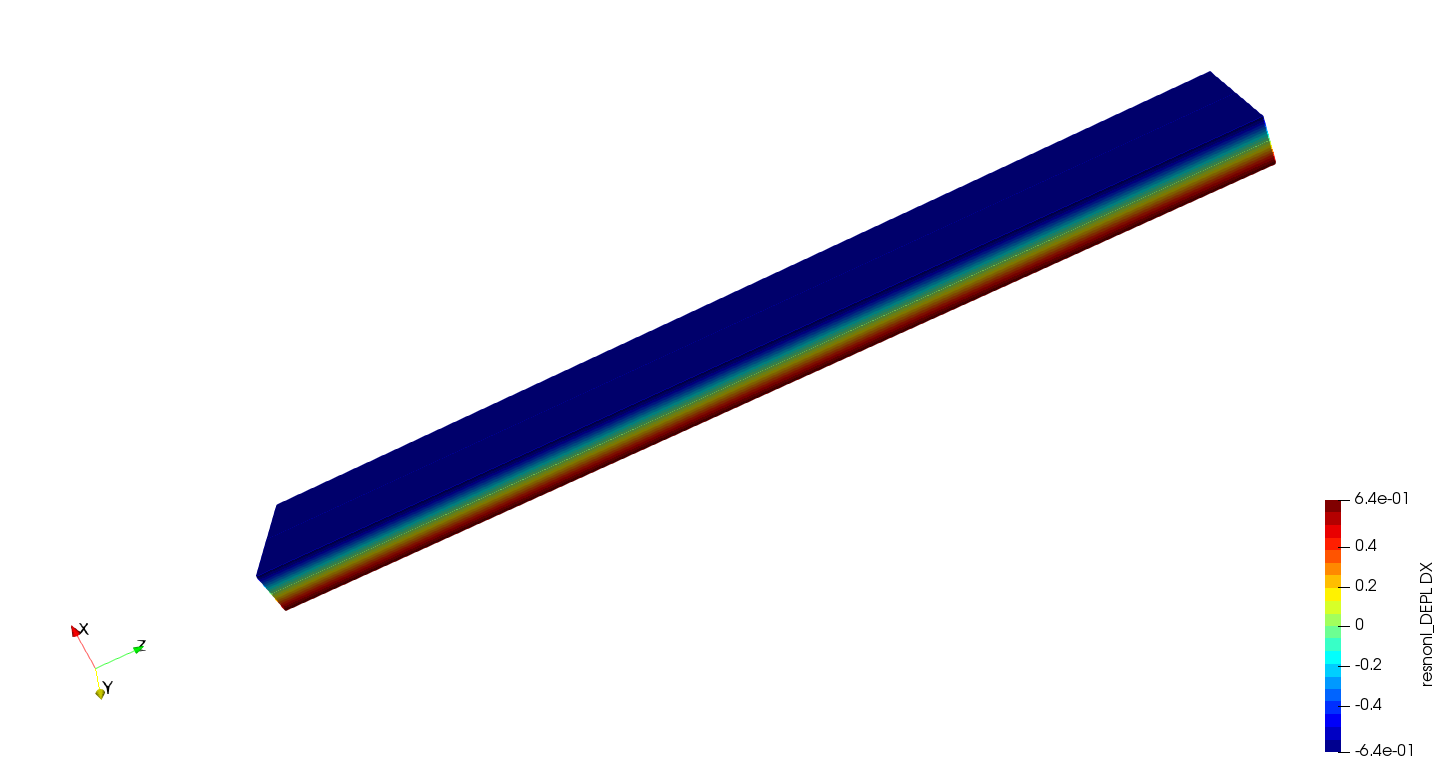
\includegraphics[width=0.9\columnwidth]{fig/dispX.png}
	\end{minipage}
	\begin{minipage}{0.32\hsize}
		\caption{Y方向変位量:1.5(mm)\\(両方向)}
		%\label{}
		\centering
		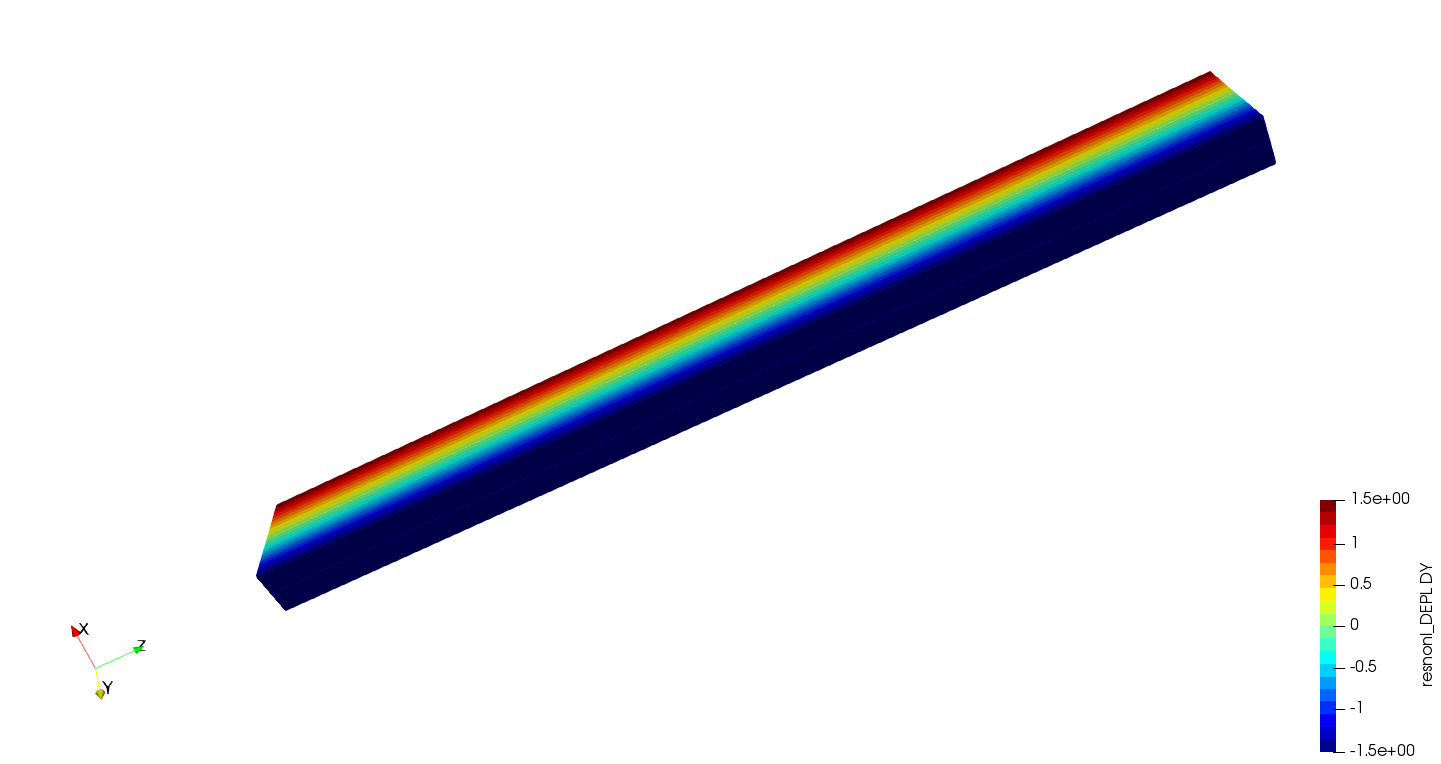
\includegraphics[width=0.9\columnwidth]{fig/dispY.png}
	\end{minipage}
	\begin{minipage}{0.32\hsize}
		\caption{Z方向変位量:34.4(mm)\\(正方向のみ)}
		%\label{}
		\centering
		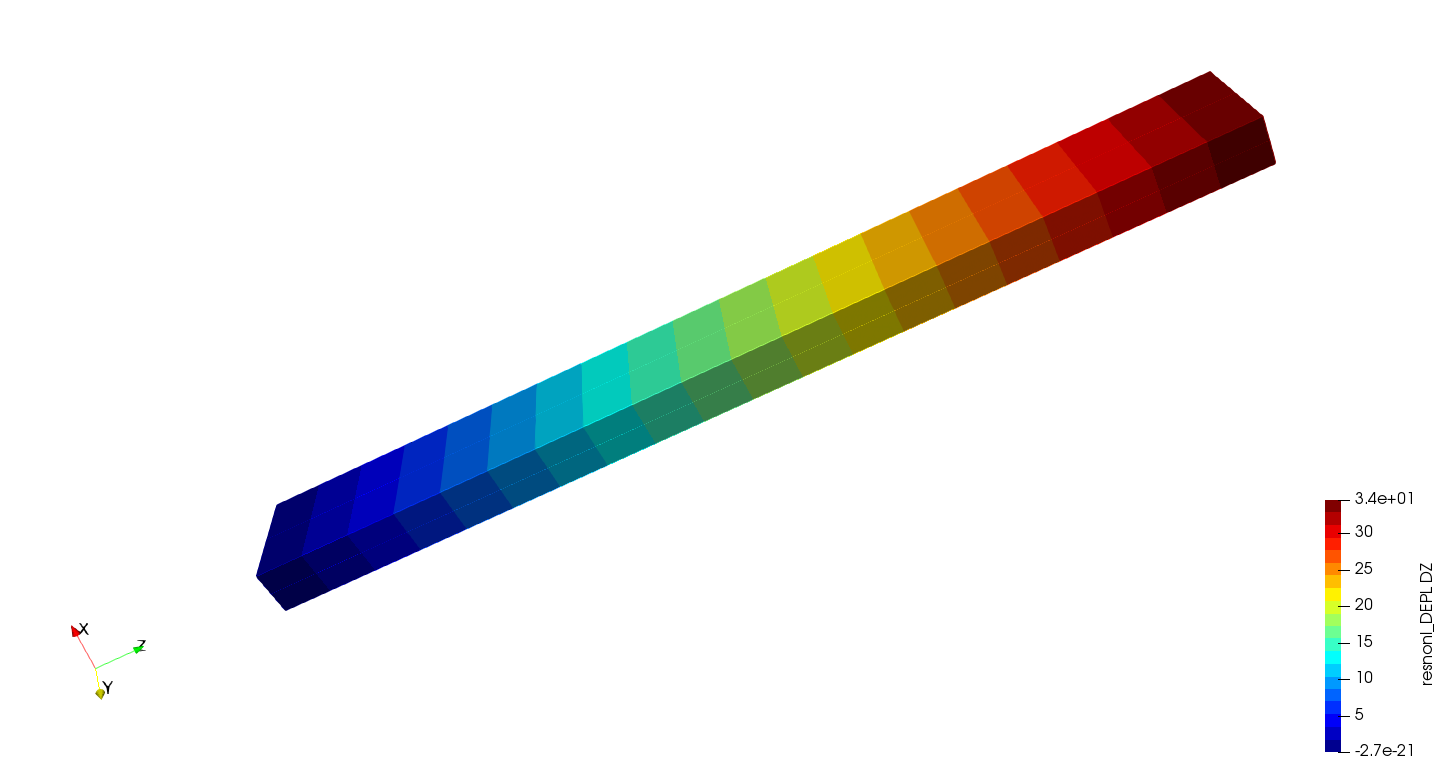
\includegraphics[width=0.9\columnwidth]{fig/dispZ.png}
	\end{minipage}
\end{figure}
ポアソン比$\nu$は、0.499にしたので、体積はほとんど変わらないと予想され、\\
変形前の体積は:
\begin{equation}
	% \label{}
	V_{0}=5\times12\times43=2,580(mm^{3})
\end{equation}
変形後の体積は:
\begin{equation}
	% \label{}
	V_{def}=2(2.5-0.64)\times2(6-1.5)\times(43+34.4)=2,591(mm^{3})
\end{equation}
体積変化は:11($mm^{3}$)でした。
\appendix
\section{コマンドファイル}
\begin{lstlisting}[caption =コマンドファイル, label=コマンドファイル]
DEBUT(LANG='EN')

mesh = LIRE_MAILLAGE(FORMAT='MED',
                     UNITE=20)

model = AFFE_MODELE(AFFE=_F(MODELISATION=('3D', ),
                            PHENOMENE='MECANIQUE',
                            TOUT='OUI'),
                    MAILLAGE=mesh)

mater = DEFI_MATERIAU(ELAS_HYPER=_F(C01=2.3456,
                                    C10=0.709,
                                    C20=0.0,
                                    NU=0.499))

fieldmat = AFFE_MATERIAU(AFFE=_F(MATER=(mater, ),
                                 TOUT='OUI'),
                         MAILLAGE=mesh)

listr = DEFI_LIST_REEL(DEBUT=0.0,
                       INTERVALLE=_F(JUSQU_A=1.0,
                                     NOMBRE=20))

times = DEFI_LIST_INST(DEFI_LIST=_F(LIST_INST=listr),
                       METHODE='AUTO')

func = DEFI_FONCTION(NOM_PARA='INST',
                     PROL_DROITE='LINEAIRE',
                     VALE=(0.0, 0.0, 1.0, 1.0))

mecabc = AFFE_CHAR_MECA(DDL_IMPO=(_F(DZ=0.0,
                                     GROUP_MA=('Abot', )),
                                  _F(DY=0.0,
                                     GROUP_NO=('Nfixx', )),
                                  _F(DX=0.0,
                                     GROUP_NO=('Nfixy', ))),
                        MODELE=model)

mecach = AFFE_CHAR_MECA(MODELE=model,
                        PRES_REP=_F(GROUP_MA=('Atop', ),
                                    PRES=-6.0))

resnonl = STAT_NON_LINE(CHAM_MATER=fieldmat,
                        COMPORTEMENT=_F(DEFORMATION='GROT_GDEP',
                                        RELATION='ELAS_HYPER'),
                        CONVERGENCE=_F(ITER_GLOB_MAXI=20),
                        EXCIT=(_F(CHARGE=mecabc),
                               _F(CHARGE=mecach,
                                  FONC_MULT=func)),
                        INCREMENT=_F(LIST_INST=listr),
                        MODELE=model,
                        NEWTON=_F(REAC_ITER=1))

resnonl = CALC_CHAMP(reuse=resnonl,
                     CONTRAINTE=('SIGM_ELNO', 'SIGM_NOEU'),
                     CRITERES=('SIEQ_ELNO', 'SIEQ_NOEU'),
                     FORCE=('FORC_NODA', 'REAC_NODA'),
                     MODELE=model,
                     RESULTAT=resnonl)

IMPR_RESU(FORMAT='MED',
          RESU=_F(MAILLAGE=mesh,
                  NOM_CHAM=('DEPL', 'SIGM_NOEU', 'SIEQ_NOEU', 'REAC_NODA', 'FORC_NODA'),
                  RESULTAT=resnonl),
          UNITE=80)

FIN()
\end{lstlisting}
%
\clearpage
% 参考文献リスト
\begin{thebibliography}{9}
	\bibitem{CAELinux} CAELinux, 『Contrib:KeesWouters/solids/mooney-rivlin』 \href{http://www.caelinux.org/wiki/index.php/Contrib:KeesWouters/solids/mooney-rivlin}{http://www.caelinux.org/wiki/index.php/Contrib:KeesWouters/solids/mooney-rivlin}
	\bibitem{MATERIAU} EDF, 『[U4.43.01] Operator DEFI\_MATERIAU』\href{https://www.code-aster.org/V2/doc/default/en/man_u/u4/u4.43.01.pdf}{https://www.code-aster.org/V2/doc/default/en/man\_u/u4/u4.43.01.pdf}
	\bibitem{Nonlinear} EDF, 『[U4.51.11] Non linear constitutive laws』\href{https://www.code-aster.org/V2/doc/default/en/man_u/u4/u4.51.11.pdf}{https://www.code-aster.org/V2/doc/default/en/man\_u/u4/u4.51.11.pdf}
	\bibitem{law} EDF, 『[R5.03.19] Hyperelastic constitutive law for nearly incompressible material』\href{https://www.code-aster.org/V2/doc/default/en/man_r/r5/r5.03.19.pdf}{https://www.code-aster.org/V2/doc/default/en/man\_r/r5/r5.03.19.pdf}
	\bibitem{SSNV187} EDF,『[V6.04.187] SSNV187 - Validation of the law on a cube ELAS\_HYPER』\href{https://www.code-aster.org/V2/doc/default/en/man_v/v6/v6.04.187.pdf}{https://www.code-aster.org/V2/doc/default/en/man\_v/v6/v6.04.187.pdf}
	\bibitem{konwakai}CMD2012,『Salome-Meca活用研究会「非線形分科会」の活動報告』
\end{thebibliography}
All content is licensed under an open-source, 'copyleft' license: \href{https://creativecommons.org/licenses/by/4.0/deed.ja}{表示 4.0 国際 (CC BY 4.0)}
\begin{figure}[htbp]
	% 	\caption}
	% 	\label{}
	\centering
	
\includegraphics{fig/license.png}
\end{figure}
\end{document}